\chapter{Binary sequence representation}
\label{kap:kap2}

This chapter is dedicated to outlining the current state of the bit vector
implementations. Bit vector stores binary sequence supporting methods $\access$,
$\rank$ and $\select$. As we have shown in section~\ref{section:WaweletTree}, wavelet
tree can be used to build a vector for the general alphabet using the bit vector
implementation. This is, why it is of the utmost importance to dedicate time
to creating fast and efficient bit vector implementation. We start with its
succinct representation, in which we simply store bits one after another. Then we
look at the compressed representation using the method RRR. In the end, we briefly
explain what other alternatives exist for compressed bit vector implementation.

\section{Bit vector implementation}

\subsection{Rank}
\label{section:rank}

Regarding $\rank$, we are concerned with two different methods namely $\rank_0(i)$
and $\rank_1(i)$. It can be observed that in binary sequence the equation
$$\rank_1(i) = i - \rank_0(i)$$ holds. Thus, it is common to only provide
the implementation of one of them. We shall focus on $\rank_1(i)$ method. There are two
straightforward solutions we can begin with to support $\rank_1$ on a bit vector
$B$. The first one does not use any precomputing at all. Every time we want
to compute $\rank_1(i)$, we run through all bits preceding $i$-th and count all
the ones. This solution is not practical for longer bit vectors but it does not
add any additional space. The second approach is to precompute $\rank$ of every
bit. This enables us to answer $\rank_1$ in constant time -- a single table lookup.
However, the space needed to support this solution is $(n\cdot\log n)$ bits where
$n$ is the length of the bit sequence. These two solutions can be combined together
to obtain an idea of a practically interesting solution where we store the pre-computed
$\rank_1$ values only for some of the bits. At first, we choose a constant $k$ and split
bit vector into non-overlapping subsequences of $k$
bits. We name these subsequences \textit{superblocks}. We then precompute $\rank_1$
only for the beginning of every superblock. This enables us to answer $\rank_1$ in time $\BigO(k)$
as we need to only access the precomputed value and then count bits from the start of the
superblock up to the queried position. In this solution, we store $\BigO(\ceil{n/k}\log n)$
bits of memory as there is $\ceil{n/k}$ superblocks and every rank can be of size at most $n$.
This version of the implementation allows us to balance between speed and space usage using the
parameter $k$. Increasing this parameter allows us to save space. On the other hand, smaller $k$
requires less work to be done. For smaller $k$ the time of answering the query may be
dominated by two cache misses that most of the time occur when accessing the precomputed ranks
and then subsequently accessing the bits on the beginning of the superblock. Continuous linear
scan through subsequent bits in $B$ can be then very cache-friendly after the initial two cache misses.

Although this solution works well and is commonly used in practice, it is possible to
answer $\rank$ query in constant time and only sublinear space overhead. This was first
shown by \cite{okanohara2007practical}. We start as in the previous solution by splitting
the bit sequence into superblocks. This time we let the superblocks be of size $\log^2 n$
and again precompute $\rank$ for every beginning of superblock. We further divide every
superblock into blocks of size $(\log n)/2$. We precompute the $\rank$ for all of these
smaller blocks but to save space we only precompute it from the beginning of the corresponding
superblock. Now, when queried for $\rank_1$ of some position, we know in which superblock this
position is located, so we know what is the number of ones up to the beginning of the superblock.
We also precomputed what is the number of ones from the beginning of the superblock up to this
block. The last step is to find out the number of ones that are located before the index in this
block. This would be easy to do linearly in time $\BigO(\log n)$. However, we are aiming for
constant time $\rank$. Thanks to block being short there are not too many possibilities for what
this block can be so we can precompute every possible $\rank$ query inside of the every possible
block The space overhead that this solution adds consists of three parts.
Precomputed $\rank$ for every superblock. Number of superblocks is $\BigO(n/\log^2 n)$ and we
need $\BigO(\log n)$ bits to store every single $\rank$ value so the total amount is
\begin{equation}
    \BigO\left(\frac{n}{\log^2 n}\cdot \log n\right).
    \label{eq:rank_space_1}
\end{equation}
Number of smaller blocks is $\BigO(n/\log n)$ but now, every block stores precomputed $\rank$
only from the beginning of superblock so this number is of size at most $\BigO(\log^2 n)$. Thus
we need at most $\BigO(\log\log^2 n)$ of bits to store it. The total amount of space for the
smaller blocks is then
\begin{equation}
    \BigO\left(\frac{n}{\lg n}\cdot \log\log^2 n\right).
    \label{eq:rank_space_2}
\end{equation}
The third part is the precomputed table where we store for every possible block and every
possible $\rank$ query over it its result. The number of different ways how the block of length
$\log(n)/2$ may look is $2^{(\log n)/2} = \sqrt{n}$. Number of possible $\rank$
queries over it is $\log n$ so this makes the table of the size
\begin{equation}
    \BigO(\sqrt{n}\log n\log\log n)
    \label{eq:rank_space_3}
\end{equation}
as every entry in the table is of size at most $\BigO(\log\log n)$. The total space used for
this solution of $\rank$ is therefore sum of \ref{eq:rank_space_1}, \ref{eq:rank_space_2} and
\ref{eq:rank_space_3}. As we may observe, every one of these is using sublinear number of bits so
we may conclude that this constant time solution for rank poses altogether just sublinear space overhead.
This solution although optimal in time complexity is not used in practice that much as it produces
3 cache misses. One for accessing the precomputed rank up to the start of the superblock, then
another one for the precomputed value of rank to the beginning of the block and in the end also one
for accessing the precomputed $\rank$ value of the block.

% TODO: ... depends on model... can be O(k/w) if we consider RAM model with w-bit registers
% that supports popcount

\subsection{Select}
\label{section:select}

It is important to note that in bit vector we are again interested in methods $\select_0$
and $select_1$. Although there is not a simple way how to convert one to another just like with
$rank$, we shall be interested mainly in $select_1$ version as the other one can be easily
implemented using the same ideas. The important property of the $\select$ method is that it
works much like an inverse to $\rank$. This is given by the fact that
                $$\rank_c(\select_c(i)) = i$$.
Thanks to $\rank$ being a nondecreasing function, it is possible to binary search for the result
of $\select_c(i)$ if we have an efficient implementation of $\rank$. This can be nicely combined
with the solution from the previous section~\ref{section:rank}. At first, we binary search for
the solution in the samples of $\rank$ stored in superblocks. When we identify the correct
superblock of length $k$ bits, we simply linearly scan for the solution. This solution is not
asking for any additional memory on top of the space used for $\rank$. The answer can be given
in time $\BigO(\log(n/k)+k)$.

There is also a constant time solution for $\select$ using the sublinear memory overhead.
This solution is just like solution for the constant time $\rank$, based on a division
to superblocks and blocks. We begin by precomputing $select(i)$ for every $i$ that is
multiple of $t_1=...$. These precomputed values take $\BigO(n/\log\log n)$ bits of space.
This also splits the bit sequence into superblocks that contain exactly $t_1$ ones (possibly
except for the last). There are
now two categories of superblocks. The ones called \textit{long} that are of size bigger
than $t_1^2$. In these superblocks, we can store the positions of ones as they are sparse
and there is not many of them. The total memory used shall be $\BigO(n/t_1^2\cdot t_1\cdot
\log n) = \BigO(n/\log\log n)$. Then there are superblocks of size smaller than $t_1^2$ called
\textit{short} that we shall solve using the same idea that we used for the original bit sequence
and superblocks. We precompute the $\select$ from the beginning of the superblock for every
multiple of $t_2=(\log\log n)^2$. These precomputed values are small as they are only from the
beginning of short superblock. Every one of these values takes $\log\log n$ of space so the
total amount of space used for the values is $\BigO(n/t_2\cdot \log\log n) = \BigO(n/\log\log n)$.
For blocks of size bigger than $t_2^2$ we shall store the positions of ones as there is not
many of them in long block. We may use the same reasoning as in the previous part to conclude
that this takes $\BigO(n/t_2^2\cdot t_2\cdot \log\log n) = \BigO(n/\log\log n)$ of bits. To
take care of the blocks of size smaller than $t_2^2$ we can precompute a table of all the
possible ways how the block may look and all the possible $\select$ queries over it with
their responses. This is possible as $t_2^2 = o(n)$.

\section{Compressed representation}
\label{section:compressed_bv}

The main idea of \textit{RRR} is to split the bit sequence into blocks of constant length
$b$. This length is a parameter of the algorithm. After this division, instead
of storing a single block as a bit sequence, we store each block encoded as a pair
of numbers $(c, o)$. Here, $c$ labels the class of the block and $o$ an offset into
the sequence of all blocks in this particular class. In most of the implementations,
$c$ is equal to the number of ones in the block. Offset, on the other hand, is the
index of block along the sequence of all the blocks with $c$ ones that are lexicographically
sorted. Note that class $c$ contains ${b\choose c}$ blocks. The offset is then bounded by:

				$$0 \leq o < {b\choose c}$$.

The process of obtaining $c$ and $o$ from the raw representation of block is called
\textit{encoding}. The opposite process is called \textit{decoding}. Although we would
like both processes to be fast. We do the encoding just once, at the initial construction
of the bit vector. On the other hand, decoding is done any time we are accessing a particular
bit in $B$ so it is more important to optimise so that decoding is as fast as possible.

For smaller block sizes, such as $b\leq 15$, it is in most cases reasonable to
generate two helper tables. One is named $E$, used for the encoding, where we can
index using the block casted to a number and get the offset of this particular block.
The class can be computed trivially by counting a number of ones. The other table
named $D$ is two dimensional. On position $D[c][o]$ we store the block that
is associated with pair $(c, o)$. In other words, this is a block containing $c$ ones
and at the same time being $o$-th in the sequence of all lexicographically sorted
blocks containing $c$ ones. Both these tables $E$ and $D$ can be computed
by generating all the possible blocks in lexicographical order before we even
obtain the sequence that we will want to represent. After this precomputation,
the encoding and decoding of a block takes constant time.

For smaller values of $b$, it is possible to store the whole table $T$ which helps us
to encode and decode the block. For bigger $b$ it is not practical and many times
impossible to store huge helper tables $E$ and $D$. On the other hand, the bigger
block size yields a better compression because of smaller per block overhead. This limitation
is something that was to some extent overcame by \cite{navarro2012fast}. They came up with the
method we shall call \textit{on the fly-decoding}. This works by encoding and decoding without
the need for helper tables. This method instead relies on a bit by bit decoding of the block
thus taking $\BigO(b)$ time instead of a constant time lookup with the help of table.

Idea is that we are decoding the block from the beginning, bit by bit until the end. On every bit,
we consider putting a zero bit on this position and count $comb$ -- the number of all
combinations how the block can look in this scenario. If the sequence number of the block --
$o$ is bigger than this number, we know that the decoded block will have one on this place.
We proceed by subtracting the number $comb$ from $o$ and proceed sequentially further.

After slicing the sequence $B$ into blocks, we need to find a way how to store pairs $(c, o)$.
We shall store all the classes and offsets in separate arrays $C$ and $O$. The array $C$ shall
be implemented as an array of fixed length elements with a length equal to
$\ceil{\log_2(b+1)}$ bits. The array $O$ shall be on the other hand implemented as an array of
variable length elements with the size needed to store $i$-th element $O[i]$ being
$\ceil{\log_2{b\choose C[i]}}$ bits.

To provide access to the particular bit, we need to first find out at which block this bit is located.
Let this be $i$-th block. To decode the block we at first need to get corresponding $C[i]$ and
$O[i]$ and then we can use a pre-computed table $D$ that matches $(c_i, o_i)$ to the original
block. Obtaining $C[i]$ is trivial as it is at a fixed offset in memory. Getting the value of
$O[i]$ is harder as it is not at a known offset but generally on an offset that can be expressed
as $$\sum_{j=1}^{i-1} \ceil{\log_2{b\choose C[i]}}$$ but can not be precomputed. To compute it
without any precomputed information, we need to basically one by one skip over elements that come
before $O[i]$. Note that to compute the previous sum, we need only successive information from $C$
so these accesses tend to be cache-friendly and fast. However, to access the $i$-th block, we need
in the worst case to look at all the elements of $C$ and this takes $\BigO(n/b)$ time. To support
this version of access, we need to store the arrays $C, O$ and helper table $D$. We shall
now argue about the size of these structures. The size of these structures is as follows:

$C$ is array of $\ceil{n/b}$ elements of fixed size $\ceil{\log(b+1)}$.

For array $O$ we argue that its size is bounded by

\begin{align*}
    \sum_{i=1}^{n/b} \ceil{{\log b\choose c_i}}
    &\leq \sum_{i=1}^{\ceil{n/b}} \log {b\choose c_i} + \ceil{n/b} \\
    &= \log\prod_{i=1}^{\ceil{n/b}} {b\choose c_i} + \ceil{n/b} \\
    &\leq \log{n\choose \#_1(B)} + \ceil{n/b} &\leq nH_0(B) + \ceil{n/b}
\end{align*}

where $\#_1(B)$ denotes the total number of ones in $B$. We obtained (TODOsomeref) using the
observation that ${n\choose k} {m\choose \ell} \leq {n+m\choose k+\ell}$. This can be seen
when we interpret the left side of the equation as a number of ways we can choose $k$ elements
from $n$ elements and $\ell$ elements from another $m$ elements. This is all contained on the
right side of the equation that includes all these combinations. $D$ is storing $2^b$ entries
and each entry is using $b$ bits of storage.
The total space used is then $$nH_0(B) + \ceil{n/b} + \ceil{n/b} \cdot \ceil{\log(b+1)} + b2^b$$.
To speed up the process of accessing block, we shall store the pointers into every $k$-th element
of $O$. This divides the process of locating $O[i]$ into two parts. The first is to find the nearest
pointer leading to element before $i$ and then move at most $k$ places. This additional structure of
roughly $\frac{n}{bk}$ integers takes the space $\BigO(\log(n)\cdot \frac{n}{bk})$.

\begin{figure}
	\centerline{
		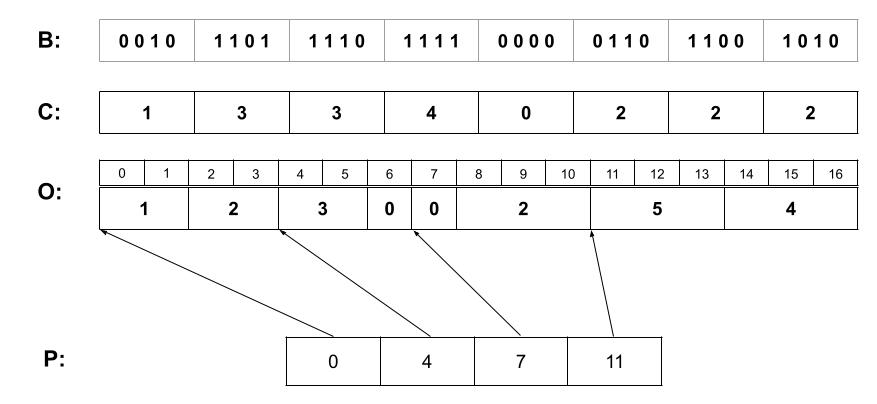
\includegraphics[width=0.9\textwidth, height=0.3\textheight]{images/rrr}
	}
	\caption[TODO]{RRR implementation. $B$ shows the original bit sequence cut to
    blocks. $C$ stores the class which is in this case number of ones in the block.
    $O$ uses variable number of bits per entry, in general, $i$-th entry uses
    $\ceil{\log_2{b\choose C[i]}}$ bits and stores the lexicographical order
    of this block in the class $C[i]$. For $k=2$ we can see a helper array $P$
    storing bit offsets into every $k$-th element namely $0, 2, 4\ldots$
	}
	\label{obr:RRRFinal}
	% source at https://docs.google.com/drawings/d/1f1M7e-dZIiIZh1RdgqnmptF3xWZBKqjms3f_aQwVMhg/edit
\end{figure}

When setting the block size to $\log(n)/2$ we obtain interesting practical results as
the total space used by our representation is equal to $nH_0(B) + o(n)$ bits. This means
that we are storing only a sublinear amount of data on top of the compressed data.

When we are interested in obtaining the best practical results, block size becomes
one of the most important parameters of RRR implementation. As we shall show in the next
chapter, bigger block size is better because of lower per bit overhead. Also, not all block
sizes are used in practice. Very often, we are interested in block sizes of the form $2^k-1$.
This is because the number of ones in block of size $2^k-1$ can be number between 0 and $2^k-1$
making this in total $2^k$ possibilities. Storing this number in the fixed bucket of size
$k$ bits makes use of all the available space. Because off this, commonly used bucket sizes in
practice are 15, 31, 63 and 127. For block size of 15 the encoding and decoding table
each occupies roughly 64kB of space. This is because every table consists of $2^{15}$ of entries
each taking 2 bytes of storage. Unfortunately, for block size of 31 these two tables would consume
roughly $2^{31}\cdot 4$ bytes of storage. That amounts to roughly 8.5GB of space and makes this approach
unusable in practice. This problem force us to use the on the fly decoding for block sizes
bigger than 15. The disadvantage of this approach is that it takes $\BigO(b)$ steps to decode the block.
Furthermore, on the fly decoding contains branches and it is hard to parallelize its steps in some meaningful
way. Overall, this makes the block size a parameter that we can adjust to balance between better space
efficiency and faster runtime performance.

\paragraph{Alternatives}
% https://github.com/simongog/sdsl-lite/blob/master/include/sdsl/sd_vector.hpp

So far we have provided just one example of the bit vector implementation.
RRR is used on sequences with low entropy, where the frequency of zeroes/ones
is shifted to one or the other side such as 20-40\% of all bits are the same.
There is also a second class of the bit vector implementations, heavily
used when the frequency of zeroes or ones is more significantly shifted.
Although we stated that RRR is used in case of shifted frequencies, when the number
of ones is very small, i.e. less than 5\% of the sequence, sparse bit vector
implementations may outperform solutions based on RRR as was observed by \cite{navarro2012fast}.
Where RRR stands out to some of its alternatives is that it is also very competitive
in cases where frequencies of zeroes and ones are similar globally, but the bit
sequence has a lot of places where locally zeroes or ones are over-represented.
Many of sparse bit vector solutions are based on the work of \cite{okanohara2007practical}.